\documentclass[10pt,a4paper,titlepage]{article}
\usepackage[latin1]{inputenc}
\usepackage{amsmath}
\usepackage{amsfonts}
\usepackage{amssymb}
\usepackage{graphicx}
\usepackage{hyperref}
\usepackage{float}
\author{Nicholas Bonham, Roy Smart}
\title{MINND Training Dataset Specification}
\begin{document}
	\maketitle
	\section{Introduction}
		It is of great interest to observe the sun and to study the explosive events that occur on its  surface. The primary goal of the \textit{MOSES} team at Montana State University is to study the transition region of the sun, and specifically to determine Doppler shifts of the formations detected in the transition region. In order to achieve this goal, the \textit{MOSES} team launched a payload on-board a Terrier-Black Brant sounding rocket to obtain solar images in three diffraction orders. The information from the solar images is convolved into what are called \textit{overlappograms}. Before any scientific analysis can be performed with the solar images, the data must be deconvolved and composed into a spectral \textit{cube}, with two spatial dimensions and one spectral dimension. This task is done by performing an \textit{inversion}. The \textit{MOSES Inversion Neural Network Design (MINND)} is a convolutional neural network designed to accomplish this effort.
		
		The motivation for \textit{MINND} is to develop a method for plaid-resistant inversion that can operate on the entire \textit{MOSES} dataset without using human designed algorithms, but instead use machine learning and training to solve the inversion problem. By offering \textit{MINND} different example problems and either rewarding or punishing the network for correct or incorrect answers, we can obtain physical results that are useful in solving the inversion problem for the full \textit{MOSES} dataset.
		
		
	\section{\textit{MOSES} Instrument}
		\subsection{Instrument Concept}
			The \textit{Multi-Order Solar EUV Spectrograph} is a sounding rocket carrying a 3-order slit-less spectrograph developed at Montana State University to produce cotemporal imaging and spectroscopy of the solar transition region and chromosphere. There are advantages to using a slit-less spectrograph versus a typical slit spectrograph as it grants the ability to create simultaneous imaging in 2D, whereas with a slit spectrograph the image is made by scanning across a field of view. Doing so intertwines temporal and spatial data, making it arduous to examine solar dynamic events.
			\begin{figure}[H]
				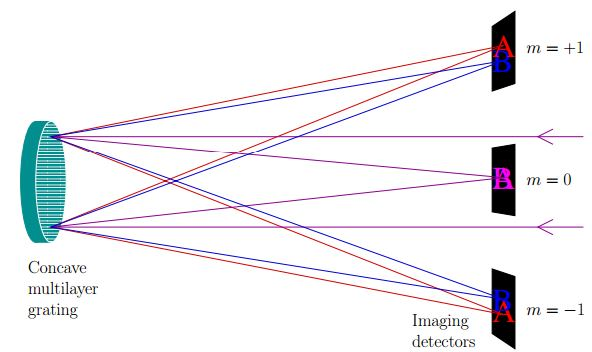
\includegraphics[scale=0.5]{mosesconcept}
				\centering
				\caption{Sketch of \textit{MOSES}.\cite{MOSESPIC}}
				\centering
			\end{figure}
			The \textit{MOSES} mission is interested in the development of the He II line and the Si XI line, with a wavelength of 303.8 {\AA} and 303.3 {\AA}, respectively \cite{MOSES}. Multiple spectral orders provide extra wavelength information, as different wavelengths are diffracted in multiple directions. Using these images, each created with a different wavelength of light, we can overlap these images to yield high spatial, spectral, and temporal resolution.
			
		\subsection{Instrument Properties}	
			The \textit{MOSES} payload is an optical instrument with an $f$/62 objective grating spectrograph operating at $\lambda$ 293-314 {\AA} in orders $n$ = $-1,0,+1$. In the outboard orders, each pixel subtends 29 m{\AA} \cite{MOSES}.
			\begin{figure}[H]
				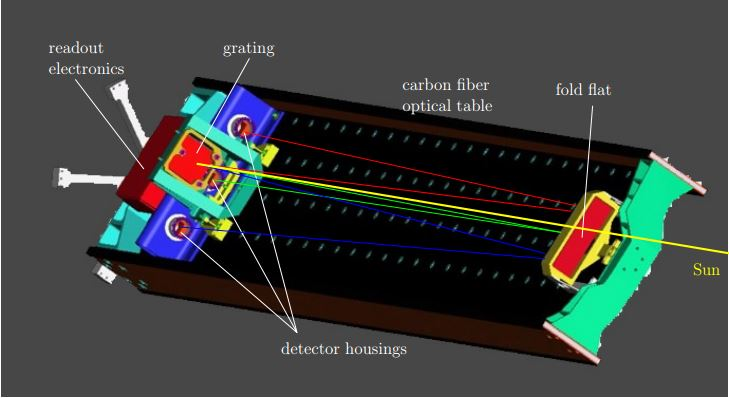
\includegraphics[scale=0.6]{moseslayout}
				\centering
				\caption{The \textit{MOSES} instrument on LOTS. The yellow, green, blue and red lines display optical rays from the Sun, rays headed to the +1,-1 and 0 orders, respectively \cite{MOSESPIC}. Not shown: baffles, shutter, LN2 plumbing, and front aperture.}
				\centering
			\end{figure}
			The entire \textit{MOSES} instrument is situated on the Lockheed Optical Table System (LOTS). Depicted in Figure 2, \textit{MOSES} consists of a primary mirror, a 10.8m spherical grating with 1160 lines/mm, and a secondary plane mirror which reflects incident light to a triad of CCD detectors near the primary mirror.
			\textit{MOSES} has a spatial resolution of 0.59''.
			Spectrally, the \textit{MOSES} instrument is interested in two specific lines; He II $\lambda$ 304 {\AA} and Si XI $\lambda$ 303.3 {\AA}. However, the instrument operates over a range of wavelengths $\lambda$ 293-314 {\AA}. The spectral resolution is 29 m{\AA}.
			
		\subsubsection{Point-Spread Function}
			\textit{MOSES} has a nontrivial point spread function. This is complicated by the fact that we cannot measure the PSF due to a lack of a collimated EUV source. Thomas Rust has estimated the PSF in the central order to be between 4 and 5 pixels FWHM from measuring compact objects in the \textit{MOSES} data.
			
		\subsubsection{Readout Electronics}
			The \textit{MOSES} readout electronics are based on that of the \textit{Hinode}/EIS system provided by Mullard Space Science Laboratory. The readout noise (pedestal) is given by a plane equation in each order.\\
			
			$n = +1:$
			\begin{equation}	
				\begin{bmatrix} x\\ y\\ constant \end{bmatrix}
				\begin{bmatrix} -2.69831\\ -1.17322\\ 515.616 \end{bmatrix}
			\end{equation}\\
			
			$n = 0:$
			\begin{equation}
			\begin{bmatrix}  x\\ y\\ constant \end{bmatrix}
			\begin{bmatrix} -3.14002\\ 1.64873\\ 381.320 \end{bmatrix}
			\end{equation}\\
			
			$n = -1:$
			\begin{equation}
			\begin{bmatrix}  x\\ y\\ constant \end{bmatrix}
			\begin{bmatrix} -1.78443\\ 0.932205\\ 486.301 \end{bmatrix}
			\end{equation}\\
			
			The CCDs on the \textit{MOSES} instrument are 1024$\times$2048 pixels. Since the size of the \textit{MOSES} CCDs along the dispersion direction (2048) is much larger than that of \textit{IRIS}, our neural network will be designed to invert only a small portion of the field of view.

			
	\section{\textit{IRIS} Instrument}
		\subsection{Instrument Concept}`
			 The \textit{Interface Region Imaging Spectrograph (IRIS)} is a small explorer mission designed by the Lockheed Martin Solar Astrophysics Laboratory (LMSAL) and launched in June of 2013. The \textit{IRIS} science motivation is to continuously observe and understand the solar atmosphere by obtaining high resolution UV images from a Slit-Jaw Spectrograph. Designed to observe the Sun for 7-8 months without obstruction, \textit{IRIS} was launched to a sun-synchronous orbit at a height of 620$\times$670 km. \textit{IRIS} obtains UV spectra and images focused on the chromosphere and transition region in two pass-bands around 1400{\AA} and 2800{\AA} \cite{ITN1}.
			 
		\subsection{Instrument Properties}
			The \textit{IRIS} instrument is comprised of a 19-cm  Cassegrain telescope with four 2061$\times$1056 CCDs and 0.16'' pixels, a 0.33'' wide and 175'' long slit spectrograph that captures FUV from 1332 {\AA} to 1358 {\AA} and NUV from 2783 {\AA} to 2835 {\AA}. Also, a slit-jaw imager including four passbands that cover a field of view of 175''$\times$175'' \cite{IRIS}. The CCDs on-board \textit{IRIS}  have a full well of 150,000 electrons and a camera readout noise of $<$20 e$^-$. 
			
				\begin{figure}[H]
					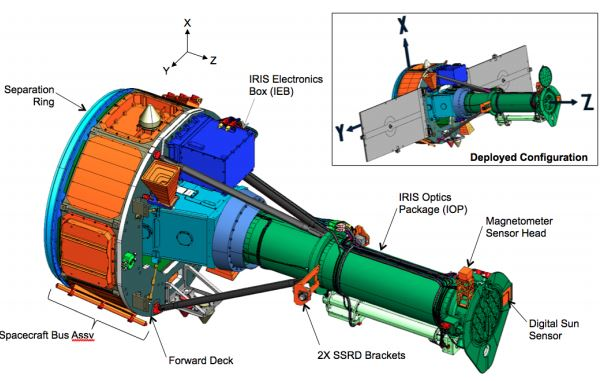
\includegraphics[scale=0.6]{iris}
					\centering
					\caption{Layout of \textit{IRIS} Instrument}
					\centering
				\end{figure}
		
			For all spectrograph passbands, the spatial resolution of \textit{IRIS} is 175 arcsec and for all slit-jaw channels, the spatial range is 175$\times$175 arcsec \cite{ITN1}. Spatial resolution is 0.33 arcsec (FUV) and 0.4 arcsec (NUV). Each pixel is 0.166 arcsec spatially. The spectral resolution in pixels is 12.8 m{\AA} for the FUV spectrograph and 25.6 m{\AA} for the NUV spectrograph.
			
			\subsubsection{Readout Electronics}
			The CCD properties of \textit{IRIS} are given in figure 3. These quantities are properties derived from dark exposures and flat images taken by \textit{IRIS} for a mercury light source with 2537 {\AA} filter.
			
			gain factor (FUV for Si IV), shoot for estimate of $\sigma_r$
				\begin{figure}[H]
					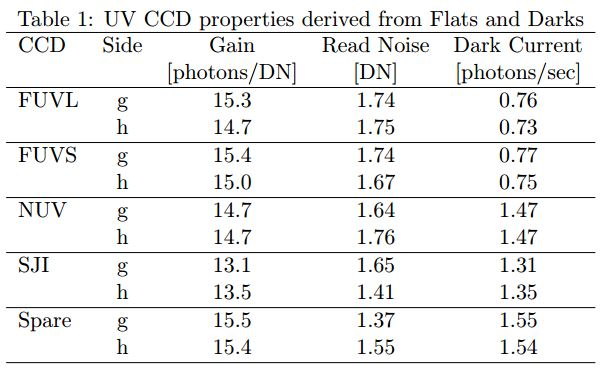
\includegraphics[scale=0.6]{gaintable}
					\centering
					\caption{UV CCD Properties \cite{ITN25}}
					\centering
				\end{figure}
			
			\subsubsection{\textit{IRIS} Database Format}
				\textit{IRIS} data are arranged into different formats, all of which are characterized by an Observation ID (OBS ID) that can be easily read to interpret data type for specific attributes. These formats are organized into a table(shown below), provided in \textit{IRIS} Technical Note 31 (ITN 31) \cite{ITN31}.\\\\
				\begin{figure}[H]
					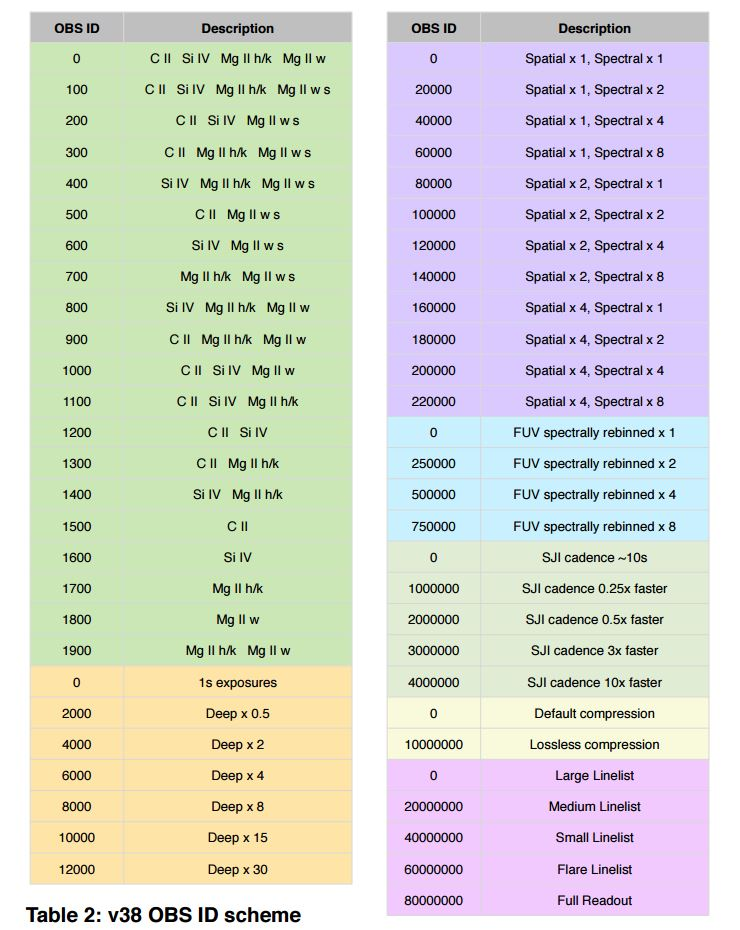
\includegraphics[scale=0.62]{obsid}
					\centering
					\caption{Table from ITN 31 showing OBSIDs for different formatting options \cite{ITN31}.}
					\centering
				\end{figure}
			
						
				Reading the OBSID is done by observing the significant digit for the parameters described in figure 5 such as cadence, raster type, and exposure times. Each parameter contains a specific value corresponding to the image type.
				
	\section{Dataset Preparation}
			\subsection{Selecting \textit{IRIS} Images}
				\label{IRIS Image}
			\subsubsection{\textit{IRIS} Image Requirements}
			
					In order for \textit{IRIS} images to be utilized in the \textit{MINND} dataset, there is a number of physical parameters that must be met so the training is applicable to the \textit{MOSES} data. The training dataset must contain spatial and spectral images at a formation temperature that is as close as possible to that of \textit{MOSES}. The formation temperatures are between 8.5$\times$10$\textsuperscript{5}$ K and 1.6$\times$10$\textsuperscript{5}$ K for Si IV \cite{1538-4357-477-2-L119}, and 5.0$\times$10$\textsuperscript{5}$ K for Ne VII \cite{bray2005plasma}. In addition, a spectral range greater than $\pm$300 km/s is desired for the \textit{IRIS} images in conjunction with a spatial range at least a factor of three times greater than that of the necessary spectral range, due to the properties of the inversion problem (these quantities are measured in pixels). To apply the point spread function appropriately, the spatial and spectral resolution of the images need to be exceeding the resolution of \textit{MOSES}. Finally, the \textit{IRIS} images needs to have a signal-to-noise ratio of at least 10, to ensure that they are quality images that can be implemented in the \textit{MINND} training dataset. 
								 
					\begin{figure}[H]
						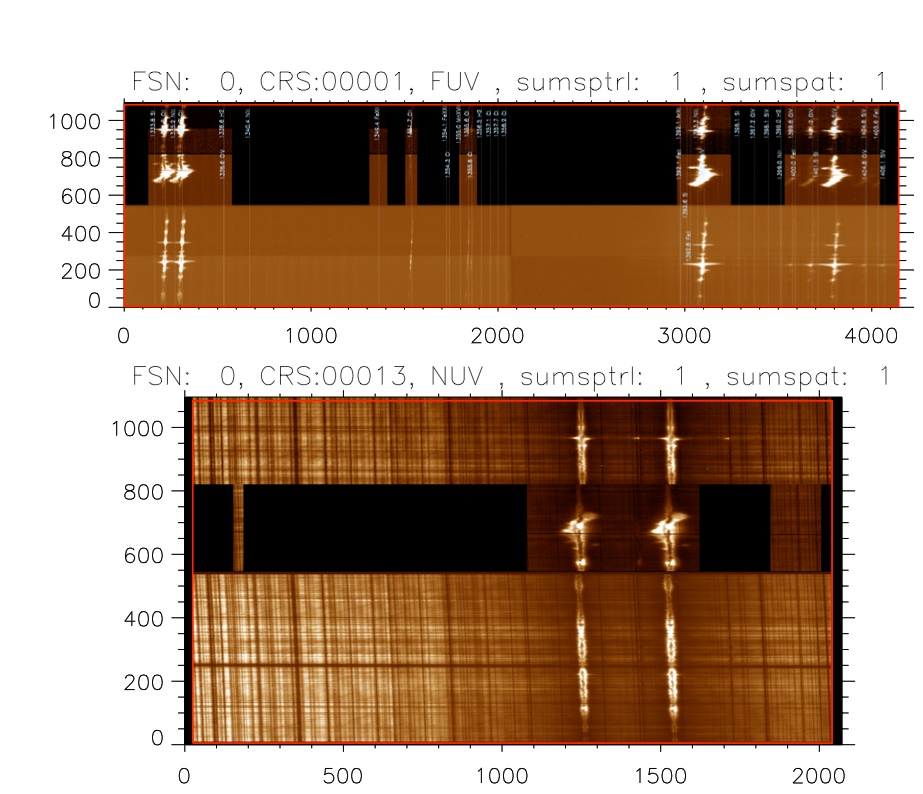
\includegraphics[scale=0.46]{IRISsample}
						\centering
						\caption{Sample \textit{IRIS} Image}
						\centering
					\end{figure}

			\subsubsection{Determining SNR}
				An expression to determine the Signal-to-Noise Ratio (SNR) is given by 
				\begin{equation}
					\text{SNR} = \frac{I j}{ \sqrt{j I + j^2 \sigma_R^2}}
				\end{equation}
				where $I$ is the median intensity, $j$ is the gain of the \textit{IRIS} instrument, and $\sigma_R$ is the readout noise. All quantities should be measured in terms of data number (DN).\\
				We can determine the quantities for SNR by first finding the line core of the image. This is done by finding the index of the maximum intensity pixel in each row of an \textit{IRIS} image. The median location of the max pixel is used to draw the line core. $I$ is the average datanumber along the line core. The images are spatial and spectral in dimension and span a range of time. To find the readout noise we select a small, quiet area with no activity and then extrude that over all time. The 1 dimensional array of the quiet area can then be used to determine the readout noise of the instrument. To do this, work out the standard deviation of the 1-dimensional array, this is the readout noise, $\sigma_R$. The gain of the \textit{IRIS} instrument in an intrinsic property that can be found in \textit{IRIS} Technical Note 25.\\

				The \textit{IRIS} data we select will be labeled ``Level A'' data.
				
			\subsection{\textit{MOSES} Forward Model}
				We further prepare the training dataset by modifying the selected IRIS images discussed in section \ref{IRIS Image} to better represent the images generated by MOSES.
			
			\subsubsection{Applying \textit{MOSES} PSF}
				As stated above, \textit{MOSES} has an asymmetric point spread function stemming from the inability to obtain a collimated EUV source. However, we can approximate this asymmetric PSF using a symmetrical 1-dimensional Gaussian PSF where the width is the average width of the \textit{MOSES} PSF (each order on \textit{MOSES} has a different average width caused by observing an object at different viewing angles). We have reduced the 3-dimensional tomography problem of \textit{MOSES} to a 2-dimensional problem with one caveat; we cannot represent the 2-dimensional PSF with only one spatial dimension. The Gaussian PSF of the above specified width is applied to the selected \textit{IRIS} images. \\
				
				This data will then be labeled ``Level B0'' data.
			
			\subsubsection{Re-sampling}
				\textit{MOSES} and \textit{IRIS} have different spatial and spectral resolutions. For the neural network to give accurate inversions, the training dataset must have the same spatial and spectral resolution. To match the resolution of the two instruments, we oversample and re-bin the Level B0 data into \textit{MOSES} pixels.\\
			
				This data will be labeled ``Level B1''. This data will form the ``truth'' dataset that will be used to train the neural network.
			
			\subsubsection{Computing Spectral Projections}
				To compute spectral projections, we will run a program named ``FOMOD'', written by Charles Kankelborg to model the optical system of the \textit{MOSES} instrument on the Level B1 data. This program will output three 1-dimensional images representing the three spectral orders captured by \textit{MOSES}.\\
				
				This dataset will be classified as ``Level B2''.

			\subsubsection{Shot Noise}
				Shot noise is an effect of the electronics on-board \textit{IRIS} that arise from the flow electric charge. This is also referred to as Poisson noise and is another type of noise that can lead to slight inaccuracies in data. To account for this, we will apply Poisson noise proportional to the mean intensity of level B2 data.
			
			\subsubsection{Read Noise}
				We wish to model the readout electronics (ROE) and its equivalent noise. To accomplish this, we apply normally distributed noise with a mean and standard deviation matched to that of the ROE. This is then applied to the training dataset.
			
	\section{Conclusion}
		At this stage of the project, Roy and I are constructing the Level A dataset. I have created a code to measure the Signal-to-Noise ratio, defined in Section 4.1.2. Our next step is to calculate the SNR using the code so we can begin the application of the \textit{MOSES} PSF and the creation of Level B0 data.
		
	\bibliographystyle{unsrt}
	\bibliography{sources}
\end{document}